\documentclass[a4paper, 12pt]{article}
\usepackage{lmodern}
\usepackage{amssymb,amsmath}
\usepackage{ifxetex,ifluatex}
\usepackage{fixltx2e} % provides \textsubscript
\ifnum 0\ifxetex 1\fi\ifluatex 1\fi=0 % if pdftex
  \usepackage[T1]{fontenc}
  \usepackage[utf8]{inputenc}
\else % if luatex or xelatex
  \ifxetex
    \usepackage{mathspec}
  \else
    \usepackage{fontspec}
  \fi
  \defaultfontfeatures{Ligatures=TeX,Scale=MatchLowercase}
\fi
% use upquote if available, for straight quotes in verbatim environments
\IfFileExists{upquote.sty}{\usepackage{upquote}}{}
% use microtype if available
\IfFileExists{microtype.sty}{%
\usepackage{microtype}
\UseMicrotypeSet[protrusion]{basicmath} % disable protrusion for tt fonts
}{}
\usepackage[left=3.5cm,right=2.5cm,top=2.5cm,bottom=2.5cm]{geometry}
\usepackage{hyperref}
\PassOptionsToPackage{usenames,dvipsnames}{color} % color is loaded by hyperref
\hypersetup{unicode=true,
            pdftitle={Regressão Quantílica},
            pdfauthor={Luiz Fernando Palin Droubi; Carlos Augusto Zilli; Murilo Damian Ribeiro; Norberto Hochheim},
            colorlinks=true,
            linkcolor=red,
            citecolor=blue,
            urlcolor=magenta,
            breaklinks=true}
\urlstyle{same}  % don't use monospace font for urls
\usepackage[style=abnt]{biblatex}

\addbibresource{bibliography.bib}
\usepackage{longtable,booktabs}
\usepackage{graphicx,grffile}
\makeatletter
\def\maxwidth{\ifdim\Gin@nat@width>\linewidth\linewidth\else\Gin@nat@width\fi}
\def\maxheight{\ifdim\Gin@nat@height>\textheight\textheight\else\Gin@nat@height\fi}
\makeatother
% Scale images if necessary, so that they will not overflow the page
% margins by default, and it is still possible to overwrite the defaults
% using explicit options in \includegraphics[width, height, ...]{}
\setkeys{Gin}{width=\maxwidth,height=\maxheight,keepaspectratio}
\IfFileExists{parskip.sty}{%
\usepackage{parskip}
}{% else
\setlength{\parindent}{0pt}
\setlength{\parskip}{6pt plus 2pt minus 1pt}
}
\setlength{\emergencystretch}{3em}  % prevent overfull lines
\providecommand{\tightlist}{%
  \setlength{\itemsep}{0pt}\setlength{\parskip}{0pt}}
\setcounter{secnumdepth}{5}
% Redefines (sub)paragraphs to behave more like sections
\ifx\paragraph\undefined\else
\let\oldparagraph\paragraph
\renewcommand{\paragraph}[1]{\oldparagraph{#1}\mbox{}}
\fi
\ifx\subparagraph\undefined\else
\let\oldsubparagraph\subparagraph
\renewcommand{\subparagraph}[1]{\oldsubparagraph{#1}\mbox{}}
\fi

%%% Use protect on footnotes to avoid problems with footnotes in titles
\let\rmarkdownfootnote\footnote%
\def\footnote{\protect\rmarkdownfootnote}

%%% Change title format to be more compact
\usepackage{titling}

% Create subtitle command for use in maketitle
\providecommand{\subtitle}[1]{
  \posttitle{
    \begin{center}\large#1\end{center}
    }
}

\setlength{\droptitle}{-2em}

  \title{Regressão Quantílica}
    \pretitle{\vspace{\droptitle}\centering\huge}
  \posttitle{\par}
  \subtitle{Quando utilizar!?}
  \author{Luiz Fernando Palin Droubi\footnote{SPU/SC,
  \href{mailto:lfpdroubi@gmail.com}{\nolinkurl{lfpdroubi@gmail.com}}} \\ Carlos Augusto Zilli\footnote{IFSC,
  \href{mailto:carloszilli@gmail.com}{\nolinkurl{carloszilli@gmail.com}}} \\ Murilo Damian Ribeiro\footnote{UFSC,
  \href{mailto:murilodamianr@gmail.com}{\nolinkurl{murilodamianr@gmail.com}}
} \\ Norberto Hochheim\footnote{UFSC,
  \href{mailto:hochheim@gmail.com}{\nolinkurl{hochheim@gmail.com}}}}
    \preauthor{\centering\large\emph}
  \postauthor{\par}
      \predate{\centering\large\emph}
  \postdate{\par}
    \date{07/01/2020}

\usepackage{expl3}
\expandafter\def\csname ver@l3regex.sty\endcsname{} 
\usepackage{wrapfig}
\usepackage[brazil]{babel}
% \usepackage{natbib}
%\usepackage{hyperref}
% \usepackage{breakurl}
\usepackage{graphicx}
\usepackage{float}
\usepackage{subfig}
\usepackage{caption}
\usepackage{lastpage}
\setlength{\parindent}{1.25cm} % Default is 15pt.
\usepackage{indentfirst}
% \usepackage{helvet}
% \renewcommand{\familydefault}{\sfdefault}
% \usepackage{newtxtext,newtxmath} % mais nova para Times.
\usepackage{mathptmx} % para Times New Roman (preferível newtxtext)
% \usepackage{Times} % para Times New Roman (obsoleto)
% \usepackage{fontspec} % para Arial e/ou Times (xelatex ou luatex)
% \setmainfont{Arial}
% \newcommand{\pkg}[1]{{\normalfont\fontseries{b}\selectfont #1}}
% \let\proglang=\textsf
% \let\code=\texttt
\newcommand{\bcenter}{\begin{center}}
\newcommand{\ecenter}{\end{center}}
\usepackage{fancyhdr}
% Turn on the style
\pagestyle{fancy}
\fancyhf{} % Clear the header and footer
\renewcommand{\headrulewidth}{0pt}
% Set the right side of the footer to be the page number
\fancyfoot[R]{\thepage~/~\pageref{LastPage}}

\begin{document}
\maketitle

\hypertarget{resumo}{%
\section*{Resumo}\label{resumo}}
\addcontentsline{toc}{section}{Resumo}

A NBR 14.653-02 \autocite{NBR1465302} recomenda que, na Engenharia de
Avaliações de imóveis urbanos, para o tratamento dos dados seja
utilizada metodologia científica, mesmo no tratamento de dados por
fatores, o que usualmente é feito através do método da regressão linear
clássica ou ordinária, ainda que a norma também cite outros métodos,
como a regressão espacial, a análise envoltória de dados e as redes
neurais artificiais. No entanto, através destes métodos, o que se obtém
são coeficientes ou fatores \textbf{médios} da contribuição de uma
característica do imóvel na formação do valor final. Ocorre que a
contribuição de uma determinada característica para a formação do valor
final dos imóveis pode ser diferente para os diferentes quantis da
distribuição de probabilidades. É possível até que uma determinada
característica que se mostre insignificante no método da regressão
linear seja significativa na regressão quantílica, já que na regressão
linear o que se estima é se, \textbf{em média}, uma determinada
característica tem influência na formação do valor total de um imóvel.
Ocorre que uma determinada característica pode influenciar positivamente
o preço de venda dos imóveis de maior valor e negativamente o preço de
venda dos imóveis de menor valor (ou \emph{vice versa}), sendo que,
\textbf{em média}, o seu efeito é nulo, o que no entanto não quer dizer
que aquela variável não tenha qualquer influência na formação de preço
dos imóveis do mercado em análise. Em suma, esta diferente contribuição
das características no valor final dos imóveis, atualmente, é ignorada
(utiliza-se apenas o valor médio), fazendo com que eventuais diferenças
nos efeitos das características em imóveis de valores diferentes sejam
negligenciadas. A regressão quantílica é um método que permite estimar a
real influência de cada característica ao longo de toda a distribuição
de probabilidades dos imóveis de um mercado, o que pode se demonstrar
útil na avaliação de imóveis urbanos em determinados mercados o que
atualmente pode passar despercebido aos olhos do avaliador acostumado
com os métodos estatísticos clássicos.

\hypertarget{introducao}{%
\section{Introdução}\label{introducao}}

\begin{quote}
What the regression curve does is give a grand summary for the averages
of the distributions corresponding to the set of of x's. We could go
further and compute several different regression curves corresponding to
the various percentage points of the distributions and thus get a more
complete picture of the set. Ordinarily this is not done, and so
regression often gives a rather incomplete picture. Just as the mean
gives an incomplete picture of a single distribution, so the regression
curve gives a correspondingly incomplete picture for a set of
distributions. \hfill --- \textcite{mosteller1977}
\autocite[apud][19]{koenker2000}
\end{quote}

Em muitas áreas da Ciência, como na Ecologia, é possível que um
pesquisador, ao analisar dados como os da figura \ref{fig:trutas} com a
utilização do consagrado método da regressão linear, chegue à conclusão
de que não há qualquer correlação entre duas variáveis, já que, pelo
estudo das variáveis, \emph{em média}, o efeito do regressor encontrado
é nulo (\(\beta = 0\)), tal como mostra a reta de regressão linear
(tracejada) na figura.

\begin{figure}[H]

{\centering \includegraphics[width=1\linewidth]{images/-000} 

}

\caption{Mudanças na densidade de trutas ($y$) em função do quociente largura/profundidade de um canal ($X$). Fonte: \textcite[413]{QReco}.}\label{fig:trutas}
\end{figure}

No entanto, como bem observaram \textcite[412-413]{QReco}, se os autores
deste estudo tivessem se baseado \emph{apenas} no método da regressão
linear, eles teriam fatalmente chegado a esta conclusão errônea. Na
realidade, porém, com o auxílio da regressão quantílica, mostrou-se que
a relação existe, porém pode ser percebida apenas nos quantis superiores
dos dados. Fisicamente, o que deve ser deduzido é que, com o aumento do
quociente largura/profundidade de um canal, limita-se a densidade de
trutas no canal. Esta limitação não é percebida nos quantis inferiores
dos dados, de maneira que, \emph{em média}, o seu efeito é nulo, mas
claramente o efeito é considerável nos quantis superiores dos dados.
Isto ocorre porque efeitos de fatores limitantes não são bem
representados pela média das distribuições de probabilidades, onde a
presença de muitos outros fatores limitantes não-medidos podem estar
presentes \cite[413]{QReco}.

O mesmo comportamento pode ou poderia ser encontrado na Engenharia de
Avaliações. Imagine-se que ao analisar um mercado de lotes urbanos o
Engenheiro de Avaliações se depare com os dados mostrados na figura
\ref{fig:urb}. Ao analisar os dados através da regressão linear à média
(reta tracejada), o Engenheiro poderia, erroneamente concluir que a área
não teria nenhum efeito sobre o valor unitário dos lotes, quando na
realidade o que ocorre é que o efeito da variável área é o de aumentar
suavemente o valor unitário dos lotes de menor valor, e diminuir de uma
forma um pouco mais agressiva o valor unitário dos lotes dos quantis
superiores.

Em suma, globalmente, o efeito médio é zero, o que não significa que a
variável não possua qualquer significância na formação de preços dos
imóveis.

A regressão quantílica permite que a influência de uma característica
qualquer de um imóvel tenha efeitos diferentes para diferentes faixas de
valores de imóveis.

\begin{figure}[H]

{\centering \includegraphics[width=1\linewidth]{images/urb-1} 

}

\caption{Dados gerados randomicamente para ilustrar a importância da regressão quantílica na Engenharia de Avaliações. Fonte: do Autor.}\label{fig:urb}
\end{figure}

\textcite{Zietz} mostram que os conflitos a respeito da contribuição de
uma determinada característica na formação dos preços de venda de
imóveis residenciais podem ser esclarecidos através da regressão
quantílica. Diferentes valores para os coeficientes de regressão linear
para algumas características podem ser encontrados ao longo da
distribuição de preços de venda de imóveis. Ou seja, algumas
características dos imóveis residenciais podem ser mais valorizados por
compradores de imóveis de mais alto valor do que por compradores de
imóveis de menor valor.

Segundo \textcite{Zietz}, variáveis como área construída, área do lote e
número de banheiros tem um impacto maior nos imóveis de maior valor de
venda, enquanto outras variáveis parecem ter um comportamento constante
para todos os preços de venda de imóveis, como garagens e distância ao
centro, entre outras.

\hypertarget{revisao-bibliografica}{%
\section{Revisão Bibliográfica}\label{revisao-bibliografica}}

\hypertarget{breve-historico}{%
\subsection{Breve Histórico}\label{breve-historico}}

Segundo \textcite[p.~347]{koenker2000}, o gráfico mais importante da
história da estatística é o gráfico de Galton, reproduzido na figura
\ref{galton}.

O gráfico ilustra o fenômeno, descoberto por Galton, da regressão à
média, cuja importância até hoje se faz presente em diversos estudos
científicos. Em estudos clínicos para a aferição do real efeito de um
novo medicamento, por exemplo, há necessidade de se estabelecerem dois
grupos de pacientes (chamados de grupos de controle e de grupo de
tratamento) para isolar os efeitos do tratamento pesquisado do efeito do
regressão à média (ou reversão à média) \autocite[ver][]{james1973}.
Nestes estudos, apenas as pessoas do grupo de tratamento realmente são
tratadas com o mediamento em teste. Desta maneira, a diferença das
médias entre os grupos é isolada da variação biológica natural e da
variação devido aos erros de aferição, que estão sujeitos à regressão à
média.

\begin{figure}
\centering
\includegraphics{image_Galton.png}
\caption{Regressão à média (Galton, 1885). Fonte:
\textcite[348]{koenker2000}\label{galton}}
\end{figure}

Segundo \textcite[p.~349]{koenker2000}, a característica essencial da
regressão linear clássica, derivada deste gráfico, é que o efeito do
covariante na variável resposta é inteiramente capturado pela expressão
abaixo, uma simples ``mudança de local'', enquanto a aleatoriedade
remanescente de \(Y\) dado \(X\) é modelada por um termo de erro aditivo
independente de \(X\).

\[\mathbb{E}(Y|X = x) = x'\beta\]

Talvez prevendo que o seu método fizesse os seus colegas estatísticos se
aterem apenas ao estudo das médias, \textcite[p.~62]{galton}
\autocite[\emph{apud}][p.~350]{koenker2000} repreendeu os seus colegas
que:

\begin{quote}
limited their inquiries to Averages, and do not seem to revel in more
comprehensive views. Their souls seem as dull to the charm of variety as
that of a native of one of our flat English counties, whose retrospect
of Switzerland was that, if the mountains could be thrown into its
lakes, two nuisances would be got rid of at once.
\end{quote}

Ironicamente, contudo, apesar da repreensão de Galton, muito
provavelmente foi o seu método o principal responsável por restringir o
escopo das investigações estatísticas à comparação de médias por décadas
\autocite[350]{koenker2000}.

Muito anterior ao descobrimento por \textcite{galton} do fenômeno da
regressão à média e ainda anterior ao descobrimento do método dos
mínimos quadrados por \textcite{legendre1805} \footnote{\textcite{gauss1809}
  ligou o método dos mínimos quadrados à distribuição normal mas a
  origem do método se deve ao trabalho pioneiro de
  \textcite{legendre1805}. Houve discordâncias entre os dois na disputa
  pela invenção do método, entre outros achados na época. Ver a este
  respeito \textcite{STIGLER197731}; \textcite{stigler1981} e
  \textcite{stigler1986}.}, Boscovich propôs, em 1760, o seguinte
problema, em busca de estimar se a hipótese elipsoidal da forma da
terra, prevista na obra-prima de \textcite{newton}, estaria correta, em
função de cinco observações do comprimento de um grau de latitude
obtidas em diferentes longitudes
\autocites[p.~353]{koenker2000}[p.~281]{tortoise}[p.~40]{stigler1986}:

Encontrar \(\hat \alpha\) e \(\hat \beta\) tais que:

\[y_i = \hat \alpha + \hat \beta x_i + \hat u_i\]

com \(\sum \hat u_i = 0\) e \(\sum |\hat u_i| = \text{min!}\).

\textcite{boscovich} propôs uma solução através de um algoritmo
geométrico. Alguns anos depois, em 1789, \textcite{laplace1789} resolveu
o problema matematicamente, nomeando o método de ``Methode de
Situation'' no que pode ser considerada a primeira análise de regressão
\autocite[281]{tortoise}.

Posteriormente, com a chegada do \emph{méthode des moindres carrés}, ou
seja, do método dos mínimos quadrados ordinários, o método dos mínimos
erros absolutos de Boscovich/Laplace ficou em segundo plano.
Posteriormente, \textcite{edgeworth1887} argumentou que, quando os erros
não seguem a lei de Gauss, a regressão à mediana poderia efetuar
melhores estimativas. Então \textcite{edgeworth1888}, relaxando a
restrição de que a soma dos resíduos seja igual a zero
(\(\sum \hat u_i = 0\)) \autocite[281]{tortoise}, propõe o primeiro o
protótipo do que viria se tornar, na década de 1940, o algoritmo
simplex, capaz de obter, de forma iterativa, o intercepto e o
coeficiente angular da reta do método dos mínimos desvios absolutos.

Na década de 40 surgiram os primeiros algoritmos simplex destinados à
otimização, algoritmos estes que se ajustam às necessidades do métodos
dos mínimos desvios absolutos, que não possui solução analítica, mas
iterativa. A primeira aplicação dos algoritmos simplex para a resolução
do método dos mínimos desvios absolutos se deve a \textcite{charnes}
\autocites[ver][281]{tortoise}[4]{conopt}.

\textcite{barrodale} propuseram a forma moderna do algoritmo simplex
que, por muitos anos e até hoje é utilizado para a minimização do erro
médio absoluto.

\textcite{koenker1978} generalizaram o problema de minimização do erro
médio absoluto, o que equivale à regressão à mediana, ao problema de
encontrar os diversos quantis de distribuição através da aplicação de
uma função de perda assimétrica, correspondente àquele quantil,
chegando-se assim à regressão quantílica.

\hypertarget{referencial-teorico}{%
\subsection{Referencial teórico}\label{referencial-teorico}}

\hypertarget{interpretacao-geometrica}{%
\subsubsection{Interpretação
Geométrica}\label{interpretacao-geometrica}}

\hypertarget{o-grafico-dual}{%
\paragraph{O gráfico dual}\label{o-grafico-dual}}

\textcite{edgeworth1888} criou o gráfico dual, ferramenta essencial para
o desenvolvimento do seu procedimento de minimização dos resíduos
absolutos. O gráfico dual nada mais é do que o gráfico, em duas
dimensões, dos parâmetros \(\alpha\) e \(\beta\) a serem estimados, com
o parâmetro \(\alpha\) nas ordenadas e o parâmetro \(\beta\) no eixo das
abscissas.

\hypertarget{algoritmo-inicial}{%
\paragraph{Algoritmo inicial}\label{algoritmo-inicial}}

\textcite{edgeworth1888} (\emph{apud} \textcite{koenker2000}, p.356)
mostrou que, para a regressão à mediana bivariada, pontos no espaço
amostral correspondem a retas no espaço paramétrico
\((x_i, y_i) \mapsto \{(\alpha, \beta): \alpha = y_i - x_i \beta\}\), e
retas através de pares de pontos no espaço amostral correspondem a
pontos (interseção das duas retas geradas pelos pontos) no espaço
paramétrico. Todos os pares de observações assim gerados produzem
\(\binom{n}{2}\) pontos no espaço paramétrico. Num espaço de \(p\)
dimensões, o número de vértices é da ordem
\(\binom{n}{p} = \mathcal{O}(n^p)\).

\textcite{edgeworth1888} então propôs um algoritmo geométrico, iniciando
em algum ponto do espaço paramétrico, mais especificamente em um ponto
de intersecção de duas retas e, iterativamente, computando a derivada
direcional da função erro absoluto (\(\ell1\)), até encontrar uma
solução ótima, ou seja, até se chegar a um ponto em que as derivadas
direcionais não sejam mais descendentes, ou seja, não haja mais nenhuma
direção onde o erro absoluto esteja diminuindo \autocite[ver][
356-358]{koenker2000}.

O procedimento acima pode ser algebricamente escrito e generalizado para
\(n\) dimensões.

\hypertarget{o-problema-de-estimacao-de-quantis-como-um-problema-de-minimizacao}{%
\subsubsection{O problema de estimação de quantis como um problema de
minimização}\label{o-problema-de-estimacao-de-quantis-como-um-problema-de-minimizacao}}

Enquanto a regressão linear, também chamada de estimador dos mínimos
(erros) quadrados, é o método análogo, para \(n\) dimensões, da média
amostral, o estimador dos mínimos erros absolutos é o método análogo à
mediana amostral em \(n\) dimensões \autocite[618]{basset}.

Desta maneira, é útil definir algebricamente a média \(\mu\) e a mediana
amostral \(Me\), como minimizações de um tipo de erro, quadrático ou
absoluto. A regressão linear e a quantílica, então, são facilmente
generalizadas pela extensão destas minimizações unidimensionais, para
\(n\) dimensões.

Pode-se demonstrar que, assim como a média aritmética \(\mu\) de uma
variável aleatória tem a propriedade de minimizar a soma dos desvios
quadráticos de cada observação em relação a ela
\autocite[50]{matloff2017}, a mediana tem a propriedade de minimizar a
soma dos desvios médios absolutos de cada observação \autocite[
260]{matloff2017}. Ou seja:

\[\mu(Y) = \mathbb{E}Y = \arg \min_c \sum_{i = 1}^n \frac{1}{n}(y_i - c)^2\]
\[Me = \arg \min_c \sum_{i = 1}^n \frac{1}{n}|y_i - c|\] Sabe-se que a
mediana de uma variável equivale ao quantil de 50\%. Assim, outros
quantis podem ser obtidos com formulação análoga à formulação acima,
porém com a aplicação de uma função de perda assimétrica
(\(\rho_\tau(.)\)) em lugar da função módulo (ver figura
\ref{fig:custo}):

\[Q_\tau(Y) = \arg \min_c \sum_{i = 1}^n \rho_\tau(y_i - c)\]

\begin{figure}[H]

{\centering \includegraphics[width=0.7\linewidth]{DmKq7} 

}

\caption{Função de perda ou custo.}\label{fig:custo}
\end{figure}

\bcenter Fonte: \textcite{qr}. \ecenter

\hypertarget{regressao-linear-e-quantilica}{%
\subsubsection{Regressão linear e
quantílica}\label{regressao-linear-e-quantilica}}

A regressão linear pode ser vista como uma forma de minimização, assim
como a média de uma população pode ser visto como o problema de
minimização descrito acima.

A diferença é que no caso da regressão linear, ao invés de minimizar em
relação a um escalar, desta vez se minimiza o erro em prever uma
variável \(Y\) em relação a uma função de outra variável \(X\),
\(f(X)\). Pode-se demonstrar que entre todas as funções \(f(X)\), a que
minimiza o erro médio quadrático de \(Y\) dado \(X\)
(\(\mathbb{E}[(Y - f(X))^2]\)) é a função de regressão
\(\mu(t) = \mathbb{E}(Y|X=t)\) \autocite[49-50]{matloff2017}. Logo,
estima-se \(\hat beta\) assim:

\[\hat \beta = \arg \min_{b \in \mathfrak{R}^p}\sum (y_i - x'_ib)^2\]

Analogamente, pode-se demonstrar que a mediana condicional é a função
que minimiza o erro médio absoluto de \(Y\) dado \(X\)
(\(\mathbb{E}(|Y-f(X)|)\)) \autocite[260-261]{matloff2017}.

Desta maneira, na regressão quantílica estima-se os coeficientes de
acordo com o seguinte problema de minimização \autocite[2]{qr40}:

\[\hat \beta(\tau) = \arg \min_{b \in \mathfrak{R}^p}\sum \rho_\tau (y_i - x'_ib)\]
Esta solução tem a propriedade de que, aproximadamente, \(\tau n\) são
positivos e \((1-\tau)n\) são negativos \autocite[3]{qr40}.

No caso particular da regressão à mediana, essa equação se reduz à:

\[\hat \beta(\tau = 0,5) = \arg \min_{b \in \mathfrak{R}^p}\sum |y_i - x'_ib|\]
A diferença, portanto, da regressão linear à média e da regressão à
mediana, pode ser escrita com a diferença da definição da norma de um
espaço vetorial, aplicada ao vetor de erros
\(\epsilon = y_i - x_i'\beta\).

No caso da regressão à mediana, essa norma é denominada norma
\(\ell_1\), enquanto na regressão à média, a norma é denominada norma
\(\ell_2\), ou norma euclidiana, de maneira que o problema de
minimização pode ser genericamente escrito como a seguir:

\[\arg \min_{b \in \mathfrak{R}^p} \sum \lVert y_i - x'_ib \rVert\]

Na regressão à mediana, a norma de um vetor \(x\) é definida da seguinte
maneira:

\[\lVert x \rVert_1 = \sum_i |x_i| = |x_1| + |x_2| + \ldots + |x_i|\]

Na regressão linear, conforme afirmou-se, a norma utilizada é a
euclidiana, assim definida:

\[\lVert x \rVert_2 = \sqrt{\left(\sum_i x_i^2\right)} = \sqrt{x_1^2 + x_2^2 + \ldots + x_i^2}\]

\hypertarget{unicidade-da-solucao}{%
\paragraph{Unicidade da solução}\label{unicidade-da-solucao}}

Pode-se demonstrar que a regressão linear, ou seja, a minimização de
\(\mathbb{E}[(Y - X\beta)^2]\) possui uma única solução e esta solução
pode ser encontrada analiticamente, bastando para isso efetuar a
derivação parcial deste termo em relação a \(\beta\) e igualando-o a
zero, obtendo-se assim uma única solução para \(\beta\) a qual
usualmente designa-se \(\hat \beta\) \autocite[ver][49-50]{matloff2017}.

O mesmo não se pode dizer da regressão à mediana e, mais genericamente,
da regressão quantílica. Nesta abordagem, há múltiplas soluções
possíveis, assim como numa amostra de tamanho par existem duas medianas
possíveis. Ainda, as soluções do problema de minimização da regressão
quantílica não podem ser encontradas analiticamente, sendo necessária a
utilização de processos iterativos para a obtenção do(s) mínimo(s).

Contudo, deve-se ter em mente que, em ambos os processos de minimização,
seja para a regressão linear ou para a regressão quantílica, trabalha-se
com apenas uma amostra da população estudada. Desta forma, os valores de
\(\hat \beta\) encontrados são apenas estimativas dos valores reais de
\(\beta\), ou seja, os valores da população.

A diferença entre as múltiplas soluções da regressão quantílica é da
ordem de \(1/n\), enquanto a amplitude da precisão da estimativa é de
tamanho \(1/\sqrt{n}\). Assim, presume-se que as múltiplas soluções
possíveis, para os casos práticos estão dentro da margem de erro para a
primeira estimativa encontrada pelo algoritmo \autocite{basset}.

\hypertarget{robustez-da-solucao}{%
\paragraph{Robustez da solução}\label{robustez-da-solucao}}

Uma das principais vantagens da regressão à mediana consiste na sua
robustez à presença de \emph{outliers}. Enquanto a solução da regressão
linear é altamente sensível à presença de eventuais \emph{outliers} na
amostra, a solução de regressão quantílica é muito menos sensível.

A figura \ref{fig:outlier1}\footnote{Fonte:
  \url{http://sfb649.wiwi.hu-berlin.de/fedc_homepage/xplore/tutorials/xaghtmlnode6.html}}
ilustra o caso típico de um \emph{outlier} presente na variáve resposta
do modelo, onde a solução da regressão quantílica se mostra totalmente
estável, pois este ponto não altera substancialmente a estimação (reta
em vermelho) da reta de regressão quantílica ``real'' (em azul). Já a
figura \ref{fig:outlier2}\footnote{Idem.} ilustra um caso onde o
\emph{outlier} é um ponto discrepante também na variável explicativa,
situação esta que não é incomum em amostras de imóveis urbanos. Neste
último caso, a solução da regressão quantílica mostra-se totalmente
sensível à influência deste ponto.

\begin{figure}[H]

{\centering \subfloat[variável resposta\label{fig:outlier1}]{\includegraphics[width=0.49\linewidth]{images/outlier_2} }\subfloat[variável explicativa\label{fig:outlier2}]{\includegraphics[width=0.49\linewidth]{images/outlier_1} }

}

\caption{Regressão quantílica: efeito de outliers na amostra.}\label{fig:outlier}
\end{figure}

\hypertarget{transformacao-e-retransformacao}{%
\paragraph{Transformação e
retransformação}\label{transformacao-e-retransformacao}}

Na regressão linear, com a aplicação do método à uma variável produto da
transformação da variável dependente original, não é suficiente a
simples retransformação dessa variável à escala original para a obtenção
da solução, já que \(f(\mathbb{E}(X)) \leq \mathbb{E}(f(X))\), devido à
desigualdade de Jensen \autocite[ver][p.~207]{moda_media_mediana}.

Já na regressão quantílica, com a aplicação de \textbf{transformações
monotônicas}, pode-se afirmar que o quantil da variável transformada
corresponde ao mesmo quantil da variável original. Assim, seja \(f(.)\)
uma transformação monotônica qualquer em \(\mathbb{R}\), e \(Q(.)\) a
função quantil, para uma variável aleatória qualquer \(Y\) pode-se
escrever:

\[Q_{f(Y)}(\tau) = f(Q_Y(\tau))\] \textcite[p.~39-40]{koenker1978}
elencam ainda quatro propriedades de equivariância para a regressão
quantílica, reproduzidas abaixo:

\[
\begin{aligned}
\hat \beta(\tau;\lambda y,X) &= \lambda \hat \beta(\tau; y, X), & \lambda \in[0,\infty), \\
\hat \beta(1-\tau;\lambda y,X) &= \lambda \hat \beta(\tau; y, X) & \lambda \in (-\infty,0],\\
\hat \beta(\tau;y + X\gamma,X)& = \hat \beta(\tau; y, X) + \gamma & \gamma \in \mathbb{R}^k,\\
\hat \beta(\tau;y,XA) &= A^{-1} \hat \beta(\tau; y, X) & A_{K \times K} \text{não-singular.}
\end{aligned}
\]

\hypertarget{eficiencia-computacional}{%
\paragraph{Eficiência computacional}\label{eficiencia-computacional}}

Segundo \textcite[p.~3]{conopt}, para amostras de tamanho menor do que
alguns milhares de dados, com algumas dúzias de parâmetros a serem
estimados, o que é hoje considerado um problema modesto pela ciência de
dados, o algoritmo de \textcite{barrodale} é considerado extremamente
eficiente.

De fato, segundo \textcite[p.~6]{conopt}, algoritmos do tipo simplex
como o de \textcite{barrolade}, ditos \emph{exterior point algorithms},
são mais eficientes para problemas de número moderado de dados e
parâmetros.

Já para a solução de problemas com maior número de dados, procedimentos
do tipo \emph{interior point algorithms}, como o de Frisch-Newton, são
substancialmente mais rápidos e precisos \autocite[6]{conopt}. De fato,
como mencionado anteriormente, com o algoritmo simplex o problema é da
ordem \(\mathcal{O}(n^p)\). Segundo \textcite[p.~369]{koenker2000}, com
a utilização de um \emph{interior point algorithm}, o problema toma a
ordem de \(\mathcal{O}(np^3\log^2n)\), ainda muito superior à ordem do
problema de mínimos quadrados, que é de ordem \(\mathcal{O}(np^2)\).

Com algum pré-processamento, é possível reduzir bastante a ordem do
problema.

Para problemas esparsos, \(i.e.\) problemas onde há um grande número de
variáveis, porém apenas algumas com valores diferentes de zero, foram
desenvolvidos outros métodos baseados em álgebra esparsa
\autocite[ver][]{koenker2005}.

Uma comparação detalhada da eficiência dos diversos métodos
computacionais com diferentes tamanhos de amostras e parâmetros pode ser
visto em \textcite{tortoise}.

Mais recentemente, com o advento do \emph{Big Data}, mesmo os algoritmos
do tipo \emph{interior point algorithms}, ainda que com uso de
pré-processamento, podem ser insuficientes. Para isto, é necessário
fazer uso do método de gradiente descendente, com o auxílio de
computação paralela \autocite[8]{qr}.

\hypertarget{estimador-de-maxima-verossimilhanca}{%
\paragraph{Estimador de máxima
verossimilhança}\label{estimador-de-maxima-verossimilhanca}}

Pode-se demonstrar que, quando a distribuição é normal, o estimador de
máxima verossimilhança para o parâmetro \(\mu\) da distribuição é a
média amostral.

Analogamente, se a distribuição dos dados for a distribuição de Laplace,
o estimador de máxima verossimilhança para o parâmetro é a mediana.

\hspace{-1.6cm}\begin{minipage}{0.5\textwidth}
\begin{figure}[H]

{\centering 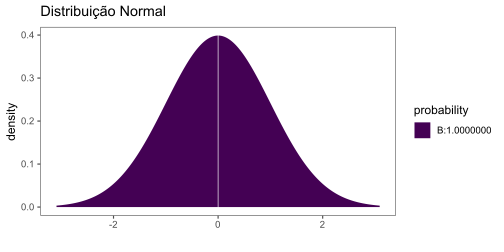
\includegraphics[width=0.7\linewidth]{images/dist_normal-1} 

}

\caption{Distribuição Normal.}\label{fig:dist_normal}
\end{figure}

\end{minipage}
\begin{minipage}{0.5\textwidth}

$$\hat \mu = \frac{1}{n}\sum x_i$$
$$\hat \sigma = \frac{1}{n-1} \sum_{i=1}^n (x_i - \hat \mu)^2$$
$$f(x|\mu, \sigma) = \frac{1}{\sigma\sqrt{2/\pi}}\exp \left (-\frac{1}{2}\frac{(x - \mu)^2}{\sigma^2} \right )$$
\end{minipage}
\hspace{-1.6cm}\begin{minipage}{0.5\textwidth}
$$\hat \mu = \arg\min_c \sum |x_i - c|$$
$$\hat \lambda = \frac{1}{n} \sum_{i=1}^n |x_i - \hat \mu| \\$$
$$f(x|\mu, \lambda) = \frac{1}{2 \lambda} \exp \left ( -\frac{|x - \mu|}{\lambda}\right )$$
\end{minipage}
\begin{minipage}{0.5\textwidth}
\begin{figure}[H]

{\centering 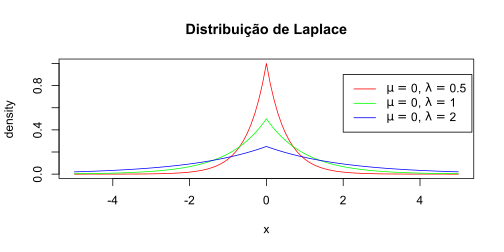
\includegraphics[width=0.7\linewidth]{images/dist_Laplace-1} 

}

\caption{Distribuição de Laplace.}\label{fig:dist_Laplace}
\end{figure}
\end{minipage}

\hypertarget{eficiencia-estatistica}{%
\paragraph{Eficiência estatística}\label{eficiencia-estatistica}}

Como mostrado no item anterior, a média é o estimador de máxima
verossimilhança quando os dados tem distribuição normal, enquanto a
mediana é o estimador de máxima verossimilhança quando os dados assumem
a distribuição de Laplace.

Na prática, no entanto, os dados não são perfeitamente normais ou
perfeitamente laplacianos, porém ajustam-se melhor ou pior a uma ou
outra, ou ainda à soma de diversas distribuições de probabilidade.

Pode-se demonstrar que, se por um lado a média amostral tem eficiência
estatística assintótica igual a 1 quando a distribuição dos dados é
normal ou gaussiana, porém ela tem menos da metade da eficiência da
mediana quando a distribuição for a distribuição de Laplace e tem
eficiência zero para a distribuição de Cauchy
\autocite[p.36]{koenker1978}.

Isto implica que, se a distribuição dos resíduos é normal, são
necessários \(\pi/2\) (1,57) vezes mais dados para que a estimativa de
\(\mu\) através da mediana seja tão eficiente quanto a estimativa
através da média. Logo, neste caso, os intervalos de confiança obtidos
para a regressão quantílica são 25\% mais largos do que os intervalos de
confiança para a regressão linear
\autocites[354]{koenker2000}[92]{dasGupta}. No entanto, se a
distribuição dos dados for a distribuição de Laplace, são necessários
duas vezes mais dados para que a média estime \(\mu\) com a mesma
precisão da mediana.

Desta maneira, quando há incerteza quanto à real distribuição dos dados,
a média, no caso escalar, ou a média condicional (regressão linear),
considerada o estimador ótimo para o caso gaussiano, pode ser preterível
à mediana, ou outros estimadores, ditos ``ineficientes''
\autocite[p.36]{koenker1978}.

A hipótese da normalidade dos dados é virtualmente preestabelecida na
comunidade científica em geral. No entanto, a verificação da normalidade
nem sempre é feita de uma maneira rigorasa. Um caso interessante ilustra
este fato: ao analisar um experimento desenhado por \textcite{pierce} em
1872 para investigar a validade da lei dos erros de Gauss, assim como a
aplicabilidade do método dos mínimos quadrados, em que este concluiu
pela justificativa da adoção da hipótese da normalidade,
\textcite{frechet} e depois \textcite{wilson} concluíram que os dados se
adaptavam melhor à primeira lei dos erros de Laplace,
\(\varphi (\epsilon) = Ce^{-|R\epsilon|}\), do que à segunda,
\(\varphi (\epsilon) = Ce^{-R^2\epsilon^2}\), \(i.e.\) à distribuição de
Gauss \autocite[62]{mim}.

Segundo \textcite[p.~618]{basset}, para qualquer distribuição de erros
em que a mediana é superior à média como um estimador de tendência
central (isto se aplica a uma enorme classe de distribuições com caudas
longas e/ou densidade máxima na mediana), o estimador de mínimos desvios
absolutos é preferível ao estimador de mínimos quadrados, apresentando
menores elipsóides de confiança assintóticamente.

\hypertarget{inferencia-e-qualidade-do-ajuste-da-regressao-quantilica}{%
\subsection{Inferência e Qualidade do ajuste da regressão
quantílica}\label{inferencia-e-qualidade-do-ajuste-da-regressao-quantilica}}

Na regressão linear, normalmente a verificação da qualidade do ajuste do
modelo é feita através do coeficiente de determinação \(R^2\), ou do
coeficiente de determinação ajustado. \textcite{r1} mostra como é
calculado a qualidade do ajuste dos dados a um modelo de regressão
quantílica.

Quando se considera o modelo de regressão linear em que os erros
apresentam distribuição normal, o coeficiente de determinação \(R^2\) é
uma medida bastante utilizada para análise da qualidade do ajuste do
modelo. Para os modelos de regressão quantílica, \textcite{r1}
propuseram uma medida semelhante ao coeficiente de determinação \(R^2\),
que permite ao pesquisador avaliar a qualidade do ajuste do modelo. Para
essa análise, considere-se um modelo linear para o quantil condicional
de \((y_i | x_i)\), com \(p\) variáveis explicativas. Teremos:

\[Q(y_i | x_i) = x_i' \beta(\tau) = x_{i1}' \beta_1(\tau) + x_{i2}' \beta_2(\tau)\]
Em que \(x_i\), \(i\)-ésima linha da matriz de planejamento \(X\), é
particionada em duas partes, aqui chamadas de \(x_{i1}\) e \(x_{i2}\) de
dimensões \(p – q\) e \(q\), respectivamente. Considere-se que
\(\hat \beta(\tau)\) é o estimador responsável por minimizar a soma dos
desvios absolutos ponderados para o modelo completo. Então teremos:

\[\hat V(\tau) = \sum_{i=1}^n \rho_\tau [y_i - x_i'\beta(\tau)]\] E
\(\tilde \beta(\tau)\), sob restrição q-dimensional
\(H_0: \beta_2(\tau)=0\), o estimador responsável por minimizar a soma
dos desvios absolutos ponderados para o modelo reduzido:

\[\tilde V(\tau) = \sum_{i=1}^n \rho_\tau [y_i - x_i' \tilde \beta(\tau)]\]
Dessa forma, o coeficiente de determinação para regressão quantílica do
modelo (1.5), pode ser definido da seguinte maneira:

\[R^1 = 1 - \frac{\hat V(\tau)}{\tilde V(\tau)}\] Considerando que
\(\tilde \beta(\tau)\) é obtido quando restringimos
\(\hat \beta(\tau)\), então \(\tilde V(\tau) \geq \hat V(\tau)\) e assim
tem-se que \(R^1 (\tau)\) terá valores dentro do intervalo
\(R^1(\tau) \in [0,1]\), sendo desta forma uma medida possível para
mensurar a qualidade do ajuste para um modelo indexado a um determinado
quantil da regressão quantílica.

\begin{quote}
Se considerarmos no vetor de parâmetros \(\beta_2(\tau)\) os
coeficientes de regressão associados a todas as variáveis explicativas
disponíveis, de forma que o modelo reduzido tenha apenas o intercepto,
então \(R^1(\tau)\) calculado se assemelha bastante ao coeficiente de
explicação \(R^2\) comumente utilizado na análise de regressão clássica
\autocite{santos2012}.
\end{quote}

Na medida em que o mede o relativo sucesso de dois modelos para a média
condicional em função de termos da variância residual, \textcite{r1}
(apud \textcite{santos2012}), nos mostram que o \(R^1(\tau)\) mede o
relativo sucesso de correspondentes modelos de regressão quantílica em
um específico quantil em função de uma apropriada soma de resíduos
absolutos ponderados. Sendo assim, o \(R^1(\tau)\) trata-se de uma
medida local de qualidade de ajuste do modelo de regressão quantílica
para um determinado quantil.

É de se esperar que o valor deste critério esteja está entre 0 e 1.
Quanto maior o coeficiente de determinação \(R^1(\tau)\), melhor a
qualidade do modelo ajustado.

A teoria relativa a regressão quantílica já evoluiu bastante desde sua
proposta original, com extensões em classes de modelos não lineares
propostos por \textcite{nlqr}. O comportamento assintótico dos
estimadores dos modelos de regressão quantílica não linear se assemelha
à teoria dos mínimos quadrados não lineares, de forma que a inferência
para regressão quantílica não linear pode ser adaptada diretamente dos
métodos destes \autocite{koenker_2005}.

\hypertarget{intervalos-de-confianca}{%
\subsubsection{Intervalos de Confiança}\label{intervalos-de-confianca}}

Segundo \textcite{qr}, é um princípio básico da Econometria que qualquer
estimador sério deve ter uma forma de verificação da sua precisão.
Existem diversas formas de se construir intervalos de confiança para a
regressão quantílica. A descrição destes métodos está fora do escopo
deste artigo. Segundo \textcite[p.~153]{qr}, as discrepâncias entre os
intervalos obtidos para a regressão quantílica e os outros métodos
disponíveis na econometria são pequenos e a inferência para a regressão
quantílica é talvez mais robusta do que as outras formas de inferência
comumente encontradas.

Uma comparação de diversos métodos de cômputo dos intervalos de
confiança para diferentes distribuições de erros pode ser encontrada em
\textcite{rqci}.

\hypertarget{aplicacoes-da-regressao-quantilica}{%
\subsection{Aplicações da regressão
quantílica}\label{aplicacoes-da-regressao-quantilica}}

Aplicações da regressão quantílica tem aplicação em especial na
Econometria, mas também nos mais diversos ramos da ciência, na solução
ou descrição de diversos problemas. Para isto, foram desenvolvidos
diferentes métodos de análise de quantis, análogos aos variados métodos
de regressão existentes para a média.

Para dados em séries temporais, foram desenvolvidos métodos para modelos
autoregressivos (AR), autoregressivos heteroscedásticos (ARCH) e ARCH
generalizados (GARCH) \autocites[ver][]{qar}{arch}{garch}. Para dados
longitudinais, ou em painel, foram desenvolvidos modelos mistos
\autocite[ver][]{koenker2003}.

Aplicações interessantes nas finanças e Econometria incluem a otimização
de portfólios de investimentos \autocite{portfolio}, e análise de dados
de desemprego \autocite{duration}.

Um resumo dos diversos métodos e aplicações da regressão quantílica
podem ser encontrados em \textcite{qr40}.

\hypertarget{estudos-de-caso}{%
\section{Estudos de Caso}\label{estudos-de-caso}}

Para os estudos de caso foram utilizados os dados disponíveis em
\textcite{hochheim}.

\hypertarget{duas-dimensoes}{%
\subsection{Duas dimensões}\label{duas-dimensoes}}

Assim como na regressão linear, é mais fácil a compreensão da regressão
quantílica através de exemplos em duas dimensões, e depois generalizar
para \(n\) dimensões.

Seja primeiramente o caso de dados heteroscedásticos. A figura
\ref{fig:qr1} ilustra a aplicação da regressão quantílica e da regressão
linear para este caso. Na figura \ref{fig:qr1}, a reta vermelha é a reta
de regressão linear entre as variáveis. A área sombreada em cinza é o
intervalo de confiança para a regressão linear @80\%. As retas azuis são
as retas de regressão quantílica para os decis \(D_1\) (0,1) a \(D_9\)
(0,9).

A regressão quantílica neste caso pode ser usada para demonstrar a não
validade dos intervalos de confiança (IC) e predição (IP) para a
regressão linear para este tipo de dados: como a variância da população
não é constante, mas aumenta com o aumento da área, as retas da
regressão quantílica se abrem. Como os intervalos de confiança e
predição na inferência clássica são calculados considerando-se que a
variância da população é constante, este efeito não se observa no
formato do IC.

\begin{figure}[H]

{\centering 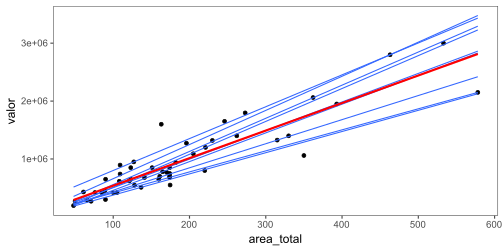
\includegraphics[width=0.7\linewidth]{images/qr1-1} 

}

\caption{Regressão Linear e Quantílica para dados heteroscedásticos.}\label{fig:qr1}
\end{figure}

Assim como na regressão linear, uma conveniente transformação das
variáveis pode ser aplicada para a obtenção da homoscedasticidade. Isto
pode ser visto na figura \ref{fig:qr2}, onde as retas para os diferentes
quantis obtidas pela regressão quantílica agora são praticamente
paralelas entre si, indicando que a heteroscedasticidade foi removida.

\begin{figure}[H]

{\centering 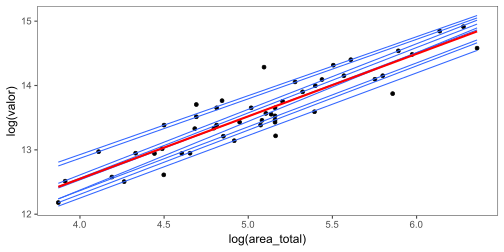
\includegraphics[width=0.7\linewidth]{images/qr2-1} 

}

\caption{Regressão Linear e Quantílica com dados transformados.}\label{fig:qr2}
\end{figure}

Os coeficientes das retas de regressão quantílica podem ser plotados
como na figura \ref{fig:coef1}. Nesta figura, a reta cheia vermelha
representa o coeficiente do modelo de regressão linear, enquanto a reta
preta pontilhada representa os vários coeficientes da regressão
quantílica. As retas vermelhas tracejadas representam o intervalo de
confiança de estimação do coeficiente de regressão linear. A área
sombreada em cinza representa os intervalos de confiança para os
coeficientes da regressão quantílica. Deve-se notar que, entre os
quantis aproximados de 0,3 e 0,55, os coeficientes da regressão
quantílica não são significantemente diferentes, estatisticamente, do
coeficiente da regressão linear.

\begin{figure}[H]

{\centering 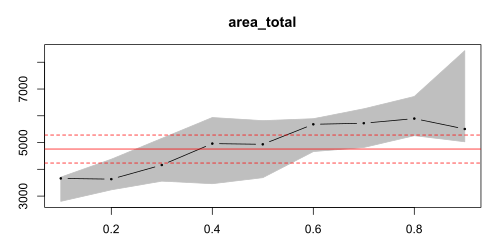
\includegraphics[width=0.7\linewidth]{images/coef1-1} 

}

\caption{Variação dos coeficientes de regressão quantílica (variáveis originais).}\label{fig:coef1}
\end{figure}

Outra forma de se analisar este gráfico é: a área total tem maior
influencia na formação de valor de um imóvel nos quantis superiores
(acima de 0,55) e menor influência nos quantis inferiores (abaixo de
0,3). Os coeficientes para os quantis 0,3; 0,5 e 0,8 podem ser vistos na
tabela \ref{tab:fits}. Para um imóvel no quantil central
(\(\tau = 0,5\)), uma unidade marginal de área adiciona aproximadamente
18,5\% mais valor do que em um imóvel nos quantis inferiores e para um
imóvel nos quantis superiores uma unidade marginal de área adiciona
aproximadamente 19,5\% mais valor do que para um imóvel no quantil
central (\(\tau = 0,5\)).

\begin{table}[!htbp] \centering 
  \caption{Comparação entre diferentes quantis da regressão quantílica.} 
  \label{tab:fits} 
\begin{tabular}{@{\extracolsep{5pt}}lccc} 
\\[-1.8ex]\hline 
\hline \\[-1.8ex] 
 & \multicolumn{3}{c}{\textit{Dependent variable:}} \\ 
\cline{2-4} 
\\[-1.8ex] & \multicolumn{3}{c}{valor} \\ 
 & $\tau=0,3$ & $\tau=0,5$ & $\tau=0,8$ \\ 
\hline \\[-1.8ex] 
 Constant & 15.397,59 & 10.855,26 & 70.373,13 \\ 
  & (63.253,00) & (69.056,43) & (102.793,74) \\ 
  & t = 0,24 & t = 0,16 & t = 0,68 \\ 
  & p = 0,81 & p = 0,88 & p = 0,50 \\ 
  & & & \\ 
 area\_total & 4.160,64 & 4.934,21 & 5.895,52 \\ 
  & (571,63) & (565,46) & (407,86) \\ 
  & t = 7,28 & t = 8,73 & t = 14,45 \\ 
  & p = 0,00$^{***}$ & p = 0,00$^{***}$ & p = 0,00$^{***}$ \\ 
  & & & \\ 
\hline \\[-1.8ex] 
Observations & 50 & 50 & 50 \\ 
\hline 
\hline \\[-1.8ex] 
\textit{Note:}  & \multicolumn{3}{r}{$^{*}$p$<$0,3; $^{**}$p$<$0,2; $^{***}$p$<$0,1} \\ 
\end{tabular} 
\end{table}

Está claro, aqui, que o efeito maior da variável área total nos quantis
superiores é devido ao efeito de um covariante, por exemplo, o padrão de
acabamento, variável omitida do modelo, que deve estar correlacionada
com a variável área total (imóveis de alto padrão usualmente contam com
área total maior e imóveis de menor área tem menor padrão de
acabamento). Mas isto serve para ilustrar bem o funcionamento da
regressão quantílica e uma de suas vantagens em relação à regressão
linear: na regressão linear, a omissão da variável padrão de acabamento,
em conjunto com um único coeficiente médio para a variável área
resultaria em um modelo viesado. Já na regressão quantílica, mesmo a
variável padrão de acabamento estando ausente, o seu efeito se faz
sentir pela mudança na magnitude do coeficiente da variável presente, ou
seja, no caso, a variável área total.

Já no caso dos dados transformados, pode-se notar na figura
\ref{fig:coef2} que para todos os quantis, os coeficientes da regressão
quantílica não podem ser considerados estatisticamente diferentes do
coeficiente da regressão linear. Também se pode notar nesta figura como
o estimador de regressão linear, para uma variável normalmente
distribuída e na ausência de heteroscedasticidade, é mais eficiente do
que o estimador da regressão quantílica, como a teoria já prevê (ver
\textcite{matloff2017}, 238).

\begin{figure}[H]

{\centering \includegraphics[width=0.7\linewidth]{images/coef2-1} 

}

\caption{Variação dos coeficientes de regressão quantílica (variáveis transformadas).}\label{fig:coef2}
\end{figure}

\hypertarget{analise-multivariada}{%
\subsection{Análise Multivariada}\label{analise-multivariada}}

Para os dados obtidos de Hochheim \autocite*[22-23]{hochheim} foram
ajustados dois modelos, um de regressão linear, com os dados saneados, e
outro de regressão quantílica, utilizando-se a totalidade dos dados,
para os decis \(D_1\) (0,1) a \(D_9\) (0,9).

Na figura \ref{fig:coefs} podem ser vistos os valores dos coeficientes
de cada variável para os diferentes quantis. Pode-se perceber, mais uma
vez, que o valor dos coeficientes da regressão quantílica não diferem
significantemente dos coeficientes da regressão linear (exceção para
alguns quantis superiores nas variáveis \texttt{area\_total} e
\texttt{padrao}).

\begin{figure}[H]

{\centering 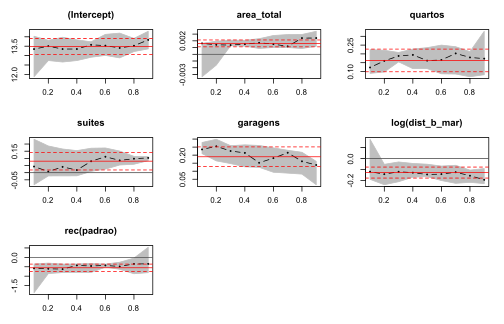
\includegraphics[width=1\linewidth]{images/coefs-1} 

}

\caption{Coeficientes de regressão linear e quantílica. Análise multivariada.}\label{fig:coefs}
\end{figure}

Na tabela \ref{tab:mfits} podem ser vistos os coeficientes e
estatísticas básicas dos modelos de regressão linear e de regressão à
mediana (quantil 0,5).

\begin{table}[!htbp] \centering 
  \caption{Comparação entre os modelos de regressão linear e regressão à mediana.} 
  \label{tab:mfits} 
\begin{tabular}{@{\extracolsep{5pt}}lcc} 
\\[-1.8ex]\hline 
\hline \\[-1.8ex] 
 & \multicolumn{2}{c}{\textit{Dependent variable:}} \\ 
\cline{2-3} 
\\[-1.8ex] & \multicolumn{2}{c}{log(valor)} \\ 
\\[-1.8ex] & \textit{OLS} & \textit{quantile} \\ 
 & \textit{} & \textit{regression} \\ 
\\[-1.8ex] & (1) & (2)\\ 
\hline \\[-1.8ex] 
 Constant & 13,564 & 13,574 \\ 
  & (13,268, 13,859) & (13,100, 14,047) \\ 
  & t = 58,847 & t = 36,732 \\ 
  & p = 0,000$^{***}$ & p = 0,000$^{***}$ \\ 
  & & \\ 
 area\_total & 0,001 & 0,002 \\ 
  & (0,001, 0,002) & (0,001, 0,003) \\ 
  & t = 5,113 & t = 2,300 \\ 
  & p = 0,00001$^{***}$ & p = 0,027$^{***}$ \\ 
  & & \\ 
 quartos & 0,164 & 0,162 \\ 
  & (0,118, 0,209) & (0,107, 0,217) \\ 
  & t = 4,626 & t = 3,788 \\ 
  & p = 0,00004$^{***}$ & p = 0,0005$^{***}$ \\ 
  & & \\ 
 suites & 0,061 & 0,080 \\ 
  & (0,018, 0,104) & (0,020, 0,139) \\ 
  & t = 1,810 & t = 1,712 \\ 
  & p = 0,078$^{***}$ & p = 0,095$^{***}$ \\ 
  & & \\ 
 garagens & 0,209 & 0,152 \\ 
  & (0,166, 0,252) & (0,075, 0,230) \\ 
  & t = 6,247 & t = 2,520 \\ 
  & p = 0,00000$^{***}$ & p = 0,016$^{***}$ \\ 
  & & \\ 
 log(dist\_b\_mar) & $-$0,141 & $-$0,146 \\ 
  & ($-$0,176, $-$0,106) & ($-$0,210, $-$0,081) \\ 
  & t = $-$5,174 & t = $-$2,904 \\ 
  & p = 0,00001$^{***}$ & p = 0,006$^{***}$ \\ 
  & & \\ 
 rec(padrao) & $-$0,563 & $-$0,459 \\ 
  & ($-$0,697, $-$0,428) & ($-$0,650, $-$0,267) \\ 
  & t = $-$5,360 & t = $-$3,070 \\ 
  & p = 0,00001$^{***}$ & p = 0,004$^{***}$ \\ 
  & & \\ 
\hline \\[-1.8ex] 
Observations & 48 & 50 \\ 
R$^{2}$ & 0,956 &  \\ 
Adjusted R$^{2}$ & 0,950 &  \\ 
Residual Std. Error & 0,136 (df = 41) &  \\ 
F Statistic & 148,921$^{***}$ (df = 6; 41) &  \\ 
\hline 
\hline \\[-1.8ex] 
\textit{Note:}  & \multicolumn{2}{r}{$^{*}$p$<$0,3; $^{**}$p$<$0,2; $^{***}$p$<$0,1} \\ 
\end{tabular} 
\end{table}

\hypertarget{estimativas}{%
\subsubsection{Estimativas}\label{estimativas}}

É interessante comparar as estimativas obtidas com os modelos de
regressão linear, com dados saneados, e o modelo de regressão à mediana,
com a totalidade dos dados. Por um lado, o modelo de regressão linear
tende a ser mais preciso para a estimação da média, como prevê a teoria.
Por outro lado, com mais dados, o modelo de regressão à mediana pode
tornar-se mais eficiente.

Deve-se levar em conta que as estimativas com o modelo de regressão
linear aqui apresentadas são para a mediana da distribuição lognormal.

Pelo modelo de regressão linear, o valor da estimativa central
encontrado foi de R\$961.660,64, com intervalo de confiança entre R\$
924.768,13 e R\$ 1.000.024,94. A amplitude do intervalo de confiança foi
de 8\%.

Já pelo modelo de regressão quantílica, o valor da estimativa central
encontrado foi de R\$946.467,87, com intervalo de confiança entre R\$
886.472,34 e R\$ 1.010.523,85. A amplitude do intervalo de confiança foi
de 13\%.

O modelo de regressão linear mostrou-se, portanto, mais eficiente do que
o modelo de regressão a mediana, apesar no menor número de dados. Os
limites inferior e superior do intervalo de predição @80\% para o modelo
de regressão linear são, respectivamente: R\$ 802.017,63 e R\$
1.153.080,88.

Para o modelo de regressão quantílica, o intervalo de predição não faz
qualquer sentido. No entanto, é possível estimar os valores diretamente
para os decis \(D_1\) e \(D_9\) da população, para efeito de comparação
com os limites do intervalo de predição para a regressão linear. Nesta
caso, os valores encontrados foram, respectivamente: R\$ 810.629,32 e
R\$ 1.186.954,14.

Podem ainda ser calculados os intervalos de confiança @80\% para as
estimativas dos decis \(D_1\) e \(D_9\).

Os limites inferior e superior do IC para o \(D_1\) são,
respectivamente: R\$ 781.253,06 e R\$ 841.110,17.

Os limites inferior e superior do IC para o \(D_9\) são,
respectivamente: R\$ 1.116.547,53 e R\$ 1.261.800,41.

A tabela abaixo resume os resultados obtidos acima: pode-se notar que há
uma melhor estimação com o método de regressão linear (IC menores).

\begin{longtable}[]{@{}llllll@{}}
\caption{Comparação dos modelos de regressão linear e regressão
quantílica.}\tabularnewline
\toprule
Método & 10\% / IP & IC inferior & Estimativa Central & IC Superior &
90\% / IP\tabularnewline
\midrule
\endfirsthead
\toprule
Método & 10\% / IP & IC inferior & Estimativa Central & IC Superior &
90\% / IP\tabularnewline
\midrule
\endhead
Regressão linear & 802.018 & 924.768 & 961.661 & 1.000.025 &
1.153.081\tabularnewline
Regressão quantílica & 810.629 & 886.472 & 946.468 & 1.010.524 &
1.186.954\tabularnewline
\bottomrule
\end{longtable}

\hypertarget{conclusao}{%
\section{Conclusão}\label{conclusao}}

A regressão quantílica é um método que deve ser considerado na
Engenharia de Avaliações, por possibilitar uma melhor descrição de todo
o mercado imobiliário, para além apenas do efeito médio obtido com a
regressão linear.

No entanto, deve ser levado em conta a distribuição dos erros do modelo:
quando os erros obedecem à lei de Gauss (ou segunda lei de Laplace),
\emph{i.e.} se os erros tem distribuição normal, como no estudo de caso
dos dados multivariados, onde se obteve normalidade através da simples
transformação da variável resposta pela função logarítmica, o método da
regressão linear é mais eficiente, até para a estimação da mediana.

Porém, deve-se levar em conta que nem sempre os dados amostrais vão se
apresentar tão bem comportados. A presença de heteroscedasticidade pode
reduzir significantemente a eficiência da estimação pelo método dos
mínimos quadrados. A ausência de normalidade também pode vir a ocorrer.
Nem sempre se pode obter a normalidade através de uma simples
transformação de variáveis. Além do mais, transformações de variáveis
distorcem o modelo, por isso são indesejáveis.

O Engenheiro de Avaliações deve estar preparado para o tratamento dos
mais diversos tipos de dados. O método da regressão quantílica pode ser
um aliado do Engenheiro de Avaliações quando a estrutura dos dados não
for a ideal, ou seja, a estrutura de erros normais e homoscedásticos,
onde a regressão linear impera.

\printbibliography[title=Referências]


\end{document}
